\documentclass[unicode, notheorems]{beamer}

\mode<presentation>
{
  \usetheme[numbers, totalnumbers]{Madrid}

  \setbeamercovered{transparent}
%
%\setbeamertemplate{footline}
%{
%  \leavevmode%
%  \hbox{%
%  \begin{beamercolorbox}[wd=.333333\paperwidth,ht=2.05ex,dp=1ex,center]{author in head/foot}%
%    \usebeamerfont{author in head/foot}\insertsection
%  \end{beamercolorbox}%
%  \begin{beamercolorbox}[wd=.333333\paperwidth,ht=2.05ex,dp=1ex,center]{title in head/foot}%
%    \usebeamerfont{title in head/foot}\insertsubsection
%  \end{beamercolorbox}%
%  \begin{beamercolorbox}[wd=.333333\paperwidth,ht=2.05ex,dp=1ex,right]{date in head/foot}%
%    \usebeamerfont{date in head/foot}\insertshortdate{}\hspace*{1em}
%    \insertframenumber{} / \inserttotalframenumber\hspace*{1ex} 
%  \end{beamercolorbox}}%
%  \vskip0pt%
%}
\setbeamertemplate{footline}{%
\hbox{%
\begin{beamercolorbox}[wd=.70\paperwidth,ht=3.25ex,dp=2ex,left,leftskip=2ex]{title in head/foot}%
    \usebeamerfont{title in head/foot}\insertshorttitle{} - \insertshortauthor
\end{beamercolorbox}%
\begin{beamercolorbox}[wd=.20\paperwidth,ht=3.25ex,dp=2ex,center]{date in head/foot}%
    \usebeamerfont{date in head/foot}\insertshortdate{}
\end{beamercolorbox}%
\begin{beamercolorbox}[wd=.10\paperwidth,ht=3.25ex,dp=2ex,right,rightskip=2ex]{date in head/foot}%
    \insertframenumber{} / \inserttotalframenumber
\end{beamercolorbox}}%
}

}
\usepackage{graphicx}
\usepackage{tikz}
%\usepackage{unicode-math}
%\setmathfont{XITS Math}
%\setmathfont[version=setB,StylisticSet=1]{XITS Math}
\usepackage{mathrsfs}

\usepackage[T2A]{fontenc}
\usepackage[utf8]{inputenc}
\usepackage[russian]{babel}
\usepackage{amsthm}
\usepackage{amsfonts}
\newcommand{\R}{\mathbb{R}}
\newcommand{\N}{\mathbb{N}}
\newcommand{\E}{\mathbb{E}}
\newcommand{\D}{\mathbb{D}}
\newcommand{\T}{\mathrm{T}}
\usepackage{amsfonts}
\usepackage{amsmath}
\usepackage{multicol}


\usepackage[T2A]{fontenc}
\ifpdf\usepackage{epstopdf}\fi

\newtheorem{theorem}{Теорема}
\newtheorem{example}{Example}
\newtheorem{definition}{Определение}
\newcommand{\scal}[2]{\left\langle #1,#2 \right\rangle}

\title{Регуляризация в регрессии}

\author{Ширинкина Дарья Андреевна, гр. 622}
\institute[СПбГУ]{Санкт-Петербургский государственный университет \\
Математико-механический факультет \\
    Статистическое моделирование
    
    \vspace{0.4cm}
    %Научный руководитель: д.ф.-м.н., профессор Ю.\,А.\,Сушков \\
    %Рецензент: д.ф.-м.н., профессор Н.\,К.\,Кривулин \\
    \vspace{0.3cm}
}
\date{
    Санкт-Петербург\\
    2017г.
}

\subject{Beamer}

\begin{document}

\begin{frame}
    \titlepage%3-5/diploma/2017m/index.html
\end{frame}


%\begin{frame}
%\frametitle{Задача}
%\textbf{Пусть}
%\begin{itemize}
%\item X --- множество объектов, Y --- множество ответов ($Y = \R$ или $Y = \R^m$);
%\item $f: X \rightarrow Y$ --- неизвестная зависимость;
%\item предполагаем, что $Y = f(X) + \varepsilon$, где $\varepsilon$ --- случайная ошибка, независящая от $X$. 
%\end{itemize}
%
%\vspace{0.5cm}
%\textbf{Дано: }
%\begin{enumerate}
%\item $\{x_1, \ldots, x_n\} \subset X$ --- обучающая выборка; 
%\item $y_i = f(x_i) + \varepsilon_i$ --- известные ответы, где $i = 1, \ldots, n$.
%\end{enumerate}
%\vspace{0.5cm}
%\textbf{Задача: }
%
%Найти решающую функцию $a: X \rightarrow Y$, приближающую $f$ на всем множестве $X$.
%
%\end{frame}

\begin{frame}
\frametitle{Задача}
\textbf{Пусть}
\begin{itemize}
\item $x_1, \ldots, x_n \in \R^p$ --- независимые одинаково распределенные случайные величины; 
\item $X = [X_1, \ldots, X_p]$, где $X_i = (x_{1i}, \ldots, x_{ni})^{\T}$, $i = 1, \ldots, p$.
\end{itemize}
\vspace{0.5cm}
Предполагаем существование неизвестной $f$ такой, что 
\[y_i = f(x_i) + \varepsilon_i,\]

где 
\begin{itemize}
\item $Y = (y_1, \ldots, y_n)^{\T} \in \R^n$;
\item $\varepsilon = (\varepsilon_1, \ldots, \varepsilon_n)$ --- независимые случайные величины;
\item $\varepsilon_i$ и $x_j$ независимы для $\forall i,j$;
\item $\E\varepsilon_i = 0$, $i = 1, \ldots, n$ и $\E\varepsilon_i^2 = \sigma^2$.
\end{itemize}
%\textbf{Дано: }
%\begin{enumerate}
%\item $\{x_1, \ldots, x_n\} \subset X$ --- обучающая выборка; 
%\item $y_i = f(x_i) + \varepsilon_i$ --- известные ответы, где $i = 1, \ldots, n$.
%\end{enumerate}
\vspace{0.5cm}
\textbf{Задача: } Оценить функцию $f$.
\vspace{0.3cm}

\end{frame}


\begin{frame}
\frametitle{Обозначения}

\textbf{Обучающая выборка:}
\begin{itemize}
\item $x_1, \ldots, x_n$ --- выборка, участвующая в оценке функции $f$ (обучающая выборка);
\item $y_i = f(x_i) + \varepsilon_i$, $i = 1, \ldots, n$.  
\end{itemize} 
\vspace{1cm}

\textbf{Тестовая выборка:}
\begin{itemize}
\item $x_1', \ldots, x_k'$ --- выборка, по которой оценивается качество оценки функции $f$ (тестовая выборка);
\item $y_i' = f(x_i') + \varepsilon_i'$, $i = 1, \ldots, k$.  
\end{itemize} 
\end{frame}

%\begin{frame}
%\frametitle{Как задаются объекты}
%
%$f_j: X \rightarrow D_j$, $j = 1, \ldots, p$ --- признаки объектов.
%
%Типы признаков:
%
%\begin{enumerate}
%\item $D_j = \{0, 1\}$ --- бинарный признак $f_j$;
%\item $|D_j| < \infty$ --- номинальный признак $f_j$;
%\item $|D_j| < \infty$, $D_j$ упорядочено --- порядковый признак $f_j$;
%\item $D_j = \R$ --- количественный признак $f_j$.
%\end{enumerate}
%
%Вектор $(f_1(x), \ldots, f_p(x))$ --- признаковое описание объекта $x \in X$.
%
%Матрица <<объекты-признаки>>
%
%\[F = || f_j(x_i)||_{n\times p} = 
%\begin{pmatrix}
%f_1(x_1) & \cdots & f_p(x_1) \\
%\cdots & \cdots & \cdots \\
%f_1(x_n) & \cdots & f_p(x_n)
%\end{pmatrix}
%.\]
%
%\end{frame}



\begin{frame}
\frametitle{Модель}

%Модель --- параметрическое семейство функций 
%
%\[A = \{ f(x, \beta) | \beta \in B\},\]
%
%где $f: X \times B\rightarrow Y$ --- фиксированная функция, 
%
%$B$ --- множество допустимых значений параметра $\beta$.
%
%\vspace{0.8cm}
Считаем, что $Y = (y_1, \ldots, y_n)^{\T}$ и $X$ --- центрированы. %$\E x_i = 0$.
\vspace{0.8cm}

\textbf{Модель многомерной линейной регрессии:}

\[y_i = f(x_i, \beta) + \varepsilon_i = \sum_{j=1}^p \beta_j x_{ij} + \varepsilon_i.\]

\textbf{Задача минимизации: } 

\[\mathrm{MSE}_{\mathrm{training}} = \frac{1}{n}\sum_{i=1}^n(y_i - \sum_{j=1}^p \beta_j x_{ij})^2 \rightarrow \min_{\beta}.\]
\vspace{0.6cm}

\textbf{Решение МНК: } $\hat{\beta} = (X^{\T}X)^{-1} X^{T}Y.$

%\begin{itemize}
%\item $f(x, \beta)$, $\beta = (\beta_1, \ldots, \beta_p)^\mathrm{T} \in \R^{p}$ --- вектор параметров модели.
%\item $f(x, \beta) \in A = \{\sum_{i=1}^p \beta_i f_i(x)| \beta = (\beta_1, \ldots, \beta_p)^\mathrm{T} \in \R^{p} \}$, где %$f_1(x), \ldots, f_p(x)$ --- числовые признаки, $x \in X$.
%\end{itemize}

\end{frame}

% Слайд: Случайный поиск с логистической кривой???

%\begin{frame}
%\frametitle{Метод обучения}
%
%Метод обучения --- это отображение вида 
%
%\[\mu: (X \times Y)^n \rightarrow A,\]
%
%которое произвольной выборке $X^n = (x_i, y_i)_{i = 1}^n$ ставит в соответствие некоторый алгоритм $a \in A$.
%
%Два этапа в задачах обучения:
%\begin{itemize}
%\item Этап обучения:
%
%метод $\mu$ по выборке $X^n$ строит алгоритм $a = \mu(X^n)$.
%
%\item Этап применения: 
%
%алгоритм $a$ для новых объектов $x$ выдает ответы $a(x)$.
%\end{itemize}
%
%\end{frame}
%
%
%\begin{frame}
%\frametitle{Функционалы качества}
%
%$\mathscr{L}(a, x)$ --- функция потерь, величина ошибки алгоритма $a \in A$ на объекте $x \in X$.
%
%Эмпирический риск --- функционал качества алгоритма $a$ на $X^n$:
%
%\[Q(a, X^n) = \frac{1}{n} \sum_{i = 1}^n \mathscr{L}(a, x_i).\] 
%
%Функции потерь для задачи регрессии:
%\begin{itemize}
%\item $\mathscr{L}(a, x)  = |a(x) - y(x)|$ --- абсолютное значение ошибки;
%\item $\mathscr{L}(a, x)  = (a(x) - y(x))^2$ --- квадратичная ошибка.
%\end{itemize}
%
%%Будем использовать для задачи МНК
%
%$y = (y_1, \ldots, y_n)$ % Что-то сделать с обозначением этого вектора, он совпадает с функцией 
%
%Функционал квадрата ошибки: 
%
%\[Q(\beta, X^n) = \sum_{i=1}^n (f(x_i, \beta) - y_i)^2 = || F\beta - y||^2 \] 
%
%\end{frame}
%
%
%\begin{frame}
%\frametitle{Задача оптимизации}
%
%Метод оптимизации эмпирического риска:
%
%\[\mu(X^n) = \arg \min_{a \in A} Q(a, X^n).\]
%
%В случае регрессии это МНК: $Q(\beta, X^n) = || F\beta - y||^2 \rightarrow \min_{\beta}$.
%
%Если модель данных с некоррелированным гауссовским шумом:
%
%\begin{align*}
%y_i = f(x_i, \beta) + \varepsilon_i, \qquad \varepsilon_i \sim N(0, \sigma^2), \qquad i = 1, \ldots, n,
%\end{align*}
%
%%\[y_i = f(x_i, \beta) + \varepsilon_i,\] \[\varepsilon_i \sim N(0, \sigma^2)\], $i = 1, \ldots, n,$  
%
%то метод МНК совпадает методом максимального правдоподобия (ММП): 
%
%\[L(\varepsilon_1, \ldots, \varepsilon_n| \beta) = \prod_{i = 1}^n \frac{1}{\sigma_i\sqrt{2\pi}} exp(-\frac{1}{2\sigma_i^2}\varepsilon_i^2) \rightarrow \max_{\beta}\]
%
%\[-ln(L(\varepsilon_1, \ldots, \varepsilon_n| \beta)) = const(\beta) + \frac{1}{2} \sum_{i = 1}^n \frac{1}{\sigma_i^2}(f(x_i, \beta) - y_i)^2 \rightarrow \min_{\beta}\]
%
%
%\end{frame}
%
%
%\begin{frame}
%\frametitle{Способ решения оптимизационной задачи}
%
%Необходимое условие минимума в матричном виде:
%
%\[\frac{\partial Q}{\partial \beta}(\beta) = 2F^{\mathrm{T}}(F\beta - y) = 0\]
%
%Получаем нормальную систему МНК:
%
%\[F^{\T}F\beta = F^{\T}y,\]
%
%где матрица $F^{\T}F$ --- матрица размера $p \times p$. 
%
%\vspace{0.8cm}
%
%\textbf{Решение системы:} $\hat{\beta} = (F^{\mathrm{T}}F)^{-1} F^{\mathrm{T}}y = F^{+}y$, где $F^{+}$ --- псевдообратная матрица.
%
%%если матрица $F^{\T}F$ невырожденная, то система имеет единственное решение  
%
%%(расписать подробнее)
%
%%сказать про интерпретацию
%
%\end{frame}
%
%\begin{frame}
%\frametitle{Сингулярное разложение}
%Произвольная $n \times p$ матрица представима в виде сингулярного разложения
%
%\[F = VDU^{\T}.\]
%
%Основные свойства сингулярного разложения:
%\begin{enumerate}
%\item $n \times p$-матрица $V = (V_1, \ldots, V_p)$ ортогональна, $V^{\T}V = I_n$, столбцы $V_j$ --- собственные вектора матрицы $FF^{\T}$;
%\item $p \times n$-матрица $U = (U_1, \ldots, U_n)$ ортогональна, $U^{\T}U = I_p$, столбцы $U_j$ --- собственные вектора матрицы $F^{\T}F$;
%\item $p \times p$-матрица $D$ диагональна $ D = diag(\sqrt{\lambda_1}, \ldots, \sqrt{\lambda_p})$ ортогональна, $\lambda_j\geq 0$ --- собственные значения матриц $F^{\T}F$ и $FF^{\T}$.
%\end{enumerate}
%
%\end{frame}
%
%\begin{frame}
%\frametitle{Решение МНК через сингулярное разложение}
%Вектор $\hat{\beta}$ --- МНК решение.
%
%\[F^{+} = (UDV^{\T} VDU^{\T})^{-1} UDV^{\T} = UD^{-1} V^{\T} = \sum_{j=1}^{p} \frac{1}{\sqrt{\lambda_j}}U_jV_j^{\T}\]
%
%\[\hat{\beta} = F^{+}y = UD^{-1}V^{\T}y = \sum_{j=1}^p \frac{1}{\sqrt{\lambda_j}} U_j(V_j^{\T}y)\]
%
%\[F\hat{\beta} = DU^{\T } UD^{-1}V^{\T}y =  VV^{\T}y = \sum_{j=1}^p V_j(V_j^{\T}y) \]
%
%\[||\hat{\beta}||^2 = || D^{-1}V^{\T}y ||^2 = \sum_{j=1}^p \frac{1}{\lambda_j} (V_j^{\T}y)^2\]
%\end{frame}
%

\begin{frame}
\frametitle{Проблема}

Насколько хорошо предсказывает $\hat{f}(x) = \sum_{i=1}^p \hat{\beta}_i x$?

\vspace{0.5cm}
%\[\mathrm{MSE}_{\mathrm{test}} = \frac{1}{n}\sum_{i=1}^n(y_i' - \sum_{i=1}^p \hat{\beta}_i x_i')^2\] 

\textbf{Проблема:} минимизируем $\mathrm{MSE}_{\mathrm{training}}$, но хотим минимизировать 

\[\mathrm{MSE}_{\mathrm{test}} = \frac{1}{n}\sum_{i=1}^n(y_i' - \sum_{j=1}^p \beta_j x_{ij}')^2.\]
\vspace{0.3cm}

\begin{itemize}
\item Нет гарантии, что минимум $\mathrm{MSE}_{\mathrm{training}}$ будет соответствовать минимуму $\mathrm{MSE}_{\mathrm{test}}$.
\item Когда $\mathrm{MSE}_{\mathrm{test}} \gg \mathrm{MSE}_{\mathrm{training}}  $, говорят, что происходит переобучение.
\end{itemize}



%Проблема обобщающей способности:
%\begin{itemize}
%\item будет ли $a = \mu(X^n)$ приближать функцию $y$ на всем $X$?
%\item будет ли $Q(a, X^n)$ мало на новых данных --- контрольной выборке $X^k = (x'_i, y'_i)_{i=1}^k$, $y'_i = y(x'_i)$?
%\end{itemize}
%
%Переобучение --- это когда $Q(\mu(X^n), X^k) \gg Q(\mu(X^n), X^n)$


% y - это вектор!!! может сделать Y??
%Пусть $\hat{y} = \hat{f}(x) + \varepsilon$ и $\hat{f}$ --- оценка $f$.
%\[\E(y - \hat{y})^2 = \E[f(x) + \varepsilon - \hat{f}(x)]^2 = (f(x) - \hat{f}(x))^2 + Var(\varepsilon)\]


\end{frame}

\begin{frame}
\frametitle{Проблема}

%\textbf{Итог:} метод дает небольшое значение $Q(a, X^n)$ для обучающей выборки, но большое для тестовой. Происходит переобучение, то есть $Q(\mu(X^n), X^k) \gg Q(\mu(X^n), X^n)$.

%\vspace{0.3cm}
Пусть
\begin{itemize}
\item $x_i'$ --- реализация случайной величина из тестовой выборки;
\item $y_i' = f(x_i') + \varepsilon_i'$ --- известное значение.
\end{itemize}

\[\E(y_i' - \hat{f}(x_i'))^2 = Var(\hat{f}(x_i')) + (Bias(\hat{f}(x_i')))^2 + Var(\varepsilon_i').\]

\vspace{0.8cm}
\begin{itemize}
\item Как правило, при увеличении сложности метода (увеличение числа параметров) дисперсия будет увеличиваться, а смещение будет уменьшаться.
\item Введение небольшого смещения в оценке может привести к значительному уменьшению дисперсии и тем самым уменьшению $\mathrm{MSE}_{\mathrm{test}}$.  
\end{itemize}


%\begin{itemize}
%\item 
%\item 
%\end{itemize}
\end{frame}


%\begin{frame}
%\frametitle{Соотношение смещения и дисперсии}
%
%\begin{figure}
%
%\begin{columns}
%
%\begin{column}{0.5\textwidth}
%\includegraphics[width=0.9\textwidth]{bias_var_trade_off.png}
%\end{column}
%
%\hspace{-2cm}
%\begin{column}{0.5\textwidth}
%\begin{itemize}
%\item Голубая кривая --- смещение в квадрате;
%\item Оранжевая кривая --- дисперсия;
%\item Красная кривая --- $\mathrm{MSE}_{\mathrm{test}}$.
%\end{itemize}
%\end{column}
%\end{columns}
%
%\end{figure}
%\end{frame}



%\begin{frame}
%\frametitle{Эмпирические оценки обобщающей способности}
%
%\textbf{Обобщающая способность метода} --- насколько метод склонен к переобучению.
%
%\vspace{0.8cm}
%\textbf{Эмпирический риск на тестовых данных (hold-out):}
%\begin{itemize}
%\item $\{x_1, \ldots, x_n\}$ --- исходная выборка размера $n$;
%\item делим случайным образом множество индексов $I = \{1, \ldots, n\}$ на два множества $I_1$ и $I_2$, для обучающей и тестовой выборки.
%\end{itemize}
%
%\[\mathrm{HO} = \sum_{i \in I_1}^n(y_i - \sum_{j=1}^p \beta_i x_{ij})^2 \rightarrow \min_{\{\beta = \beta(x_{ij}, y_i)| i \in I_2, j = 1:p\}}.\]
%\end{frame}
%
%
%\begin{frame}
%\frametitle{Эмпирические оценки обобщающей способности}
%
%\textbf{Кросс-проверка (cross-validation):}
%\begin{itemize}
%\item $\{x_1, \ldots, x_n\}$ --- исходная выборка размера $n$;
%\item делим случайным образом множество индексов $I = \{1, \ldots, n\}$ на $k$ не пересекающихся групп  $I_1, \ldots ,I_k$.
%\end{itemize}
%
%\[\mathrm{MSE}_s = \sum_{i \in I_s}^n(y_i - \sum_{j=1}^p \beta_i x_{ij})^2 \rightarrow \min_{\{\beta = \beta(x_{ij}, y_i)| i \in I \setminus I_s, j = 1:p\}},\]
%
%\[\mathrm{CV_{(k)}} = \frac{1}{k} \sum_{s = 1}^k \mathrm{MSE}_s.\]
%
%\textbf{Скользящий контроль (leave-one-out):} $k = n.$
%
%%\begin{itemize}
%%\item Эмпирический риск на тестовых данных (hold-out):
%%\[\mathrm{HO}(\mu, X^n, X^k) = Q(\mu(X^n), X^k) \rightarrow \min\]
%%\item Скользящий контроль (leave-one-out), $N = n+1$:
%%\[\mathrm{LOO}(\mu, X^N) = \frac{1}{N} \sum_{i = 1}^N \mathscr{L}(\mu(X^N\setminus \{x_i\}), x_i) \rightarrow \min\]
%%\item Кросс-проверка (cross-validation), $N = n + k$, $X^N = X^n_p\sqcup X^k_p$ :
%%\[CV(\mu, X^N) = \frac{1}{|N|} \sum_{p \in N} Q(\mu(X^n_p), X^k_p) \rightarrow \min\]
%%%\item Эмпирическая оценка вероятности переобучения:
%%%\[Q_{\varepsilon}(\mu, X^N) = \frac{1}{|N|} \sum_{p \in N}\]
%%\end{itemize}
%\end{frame}


\begin{frame}
\frametitle{Регуляризация}

\textbf{Регуляризация:} вводим ограничения на коэффициенты $\beta$.

\vspace{0.8cm}
Для чего используем регуляризацию:
\begin{itemize}
\item можем уменьшить дисперсию оценки за счет введения смещения и тем самым уменьшить $\mathrm{MSE}_{\mathrm{test}}$ (особенно, когда $p >n$);
\item можем производить отбор значимых признаков, делая коэффициенты при них равными нулю.
\end{itemize}


\end{frame}


\begin{frame}
\frametitle{Гребневая регрессия}

%Будем регулировать величину коэффициентов $\beta_i$, чтобы уменьшить их дисперсию:
Задача минимизации:

\[\sum_{i=1}^n(y_i - \sum_{j=1}^p \beta_j x_{ij})^2  + \lambda \sum_{j = 1}^p \beta_j^2 \rightarrow \min_{\beta},\]

где $\lambda \geq 0$ --- неотрицательный параметр регуляризации (tuning parameter).

\begin{itemize}
\item $\lambda\sum_{j = 1}^p \beta_j^2$ мало, когда $\beta_1, \ldots, \beta_p$ близки к нулю.
\item Когда $\lambda = 0$, то гребневая регрессия совпадает с обычной регрессией, но при $\lambda \rightarrow \infty$ коэффициенты регрессии стремятся к нулю.

\item Необходимо выбрать хорошее значение $\lambda$.
\end{itemize}

%Таким образом, параметр $\lambda$ служит для регулирования взаимодействия $||F\beta - y ||^2$


%Чем больше $\lambda$, тем коэффициенты $\beta$ стягиваются ближе к нулю.


%Смысл: уменьшить дисперсию оценок $\beta$ с помощью смещения

%Оптимизационная задача: $Q_{\lambda}(\beta)  = ||F\beta - y ||^2 + \lambda|| \beta||^2 \rightarrow \min_{\beta}$


%(см начало 6.2.1 ISLR )

%лучше признаки стандартизовать! (см 6.2.1 ISLR An Aplication to the Credit Data --- конец этого пункта, стр 217)


\end{frame}




\begin{frame}
\frametitle{Способ решения оптимизационной задачи}

Модифицированное МНК решение гребневой регрессии:
\[\hat{\beta}_{\lambda}^{R} = (X^{\mathrm{T}}X+ \lambda I_p)^{-1} X^{\mathrm{T}}Y.\]

Решение через сингулярное разложение, где $X = VDU^{\T}$:

\begin{itemize}
\item \textbf{МНК}
\[\hat{\beta} = \sum_{j=1}^p \frac{1}{\sqrt{\lambda_j}} U_j(V_j^{\T}Y);\]
\item \textbf{МНК гребневой регрессии }
\[\hat{\beta}_{\lambda}^{R} = U(D^2 + \lambda I_p)^{-1}DV^{\T}y = \sum_{j=1}^p \frac{\sqrt{\lambda_j}}{\lambda_j + \lambda} U_j(V_j^{\T}Y).\]

\end{itemize}

С помощью сингулярного разложения можно быстро выбирать параметр $\lambda$.

%Решение гребневой регрессии более устойчиво (оценки не будут сильно меняться на разных данных, если $X$ близка к вырожденной).



%\[\hat{\beta} = \sum_{j=1}^p \frac{1}{\sqrt{\lambda_j}} U_j(V_j^{\T}y)\]
%
%\[\hat{\beta}_{\lambda}^{R} = U(D^2 + \lambda I_p)^{-1}DV^{\T}y = \sum_{j=1}^p \frac{\sqrt{\lambda_j}}{\lambda_j + \lambda} U_j(V_j^{\T}y);\]
%
%
%
%\[F\hat{\beta}_{\lambda}^{R} = VDU^{\T}\hat{\beta}_{\lambda} = V diag(\frac{\lambda_j}{\lambda_j + \lambda}) V^{\T}y = \sum_{j=1}^p \frac{\lambda_j}{\lambda_j + \lambda} V_j(V_j^{\T}y);\]
%
%\[||\hat{\beta}_{\lambda}^{R}||^2 = ||(D^2 + \lambda I_p) DV^{\T}y ||^2 = \sum_{j=1}^p \frac{\lambda_j}{(\lambda_j + \lambda)^2} (V_j^{\T}y)^2.\]

\end{frame}







\begin{frame}
\frametitle{Выбор параметра регуляризации}

Как выбрать параметр $\lambda$:
\begin{itemize}
\item выбираем сетку значений $\lambda$;
\item вычисляем ошибку кросс-проверки для каждого значения $\lambda$;
\item выбираем $\lambda$ с наименьшим значением ошибки кросс-проверки;
\item перестраиваем модель со всеми наблюдениями с выбранным значением $\lambda$.
\end{itemize}

%\[X\hat{\beta}_{\lambda}^{R} = VDU^{\T}\hat{\beta}_{\lambda} = V \mathrm{diag}(\frac{\lambda_j}{\lambda_j + \lambda}) V^{\T}y = \sum_{j=1}^p \frac{\lambda_j}{\lambda_j + \lambda} V_j(V_j^{\T}y).\]

%Вычисление функционала $Q$ на контрольной выборке $X^k = (x'_i, y'_i)_{i=1}^k$:

%\[Q(\hat{\beta}_{\lambda}^{R}, X^k) = ||F'\hat{\beta}_{\lambda}^{R} - y'||^2 = ||F'U' diag(\frac{\sqrt{\lambda_j}}{\lambda_j + \lambda}) V^{\T}y - y'||^2\]



\end{frame}





\begin{frame}
\frametitle{Вероятностная интерпретация} 

\begin{itemize}
\item $\beta = (\beta_1, \ldots, \beta_p)^{\T}$ имеет априорное распределение $p(\beta)$;
\item $f(Y|X,\beta)$ --- функция правдоподобия исходных данных. 
\end{itemize}

\vspace{0.3cm}
При фиксированном $X$ апостериорное распределение $p(\beta|X,Y)$ пропорционально 
\[f(Y|X,\beta)p(\beta|X) = f(Y|X,\beta)p(\beta).\]

Предполагая, что 
\begin{enumerate}
\item линейная модель имеет независимые и нормально распределенные ошибки; 
\item $p(\beta) = \prod_{j = 1}^p g(\beta_j)$ для некоторой плотности $g$.
\end{enumerate}

%Гребневая регрессия --- это модель, где $g$ --- плотность нормального распределения с нулевым средним и дисперсией $\lambda$.
\vspace{0.5cm}
Если $g$ --- плотность $N(0,\lambda)$, то  оценка апостериорного максимума $\beta$ совпадает с решением гребневой регрессии.
%наиболее вероятное значение для \beta 

%(In fact, the ridge regression solution is also the posterior mean.)
\end{frame}


\begin{frame}
\frametitle{Смещение оценки}

Пусть $X^{\T}X = \Sigma$ и $Y = (y_1, \ldots, y_n)^{\T}$.

Оценка гребневой регрессии через МНК оценку:

\begin{align*}
\hat{\beta}_{\lambda}^R = (I_p + \lambda \Sigma^{-1})\hat{\beta}.  
\end{align*}

%\begin{align*}
%\hat{\beta}_{\lambda}^R &= (X^{\T}X + \lambda I_p)^{-1}X^{\T}Y = \\
% &= (\Sigma + \lambda I_p)^{-1} \Sigma(\Sigma^{-1}X^{\T}Y) = \\
% &= [\Sigma(I_p + \lambda\Sigma^{-1})]^{-1} \Sigma[(X^{\T}X)^{-1}X^{\T}Y] = \\
% &= (I_p + \lambda \Sigma^{-1})^{-1} \Sigma^{-1} \Sigma \hat{\beta} = \\
% &= (I_p + \lambda \Sigma^{-1})\hat{\beta}.  
%\end{align*}

Оценка гребневой регрессии имеет смещение:

\begin{align*}
\E\hat{\beta}_{\lambda}^{R} &= \E[(I_p + \lambda \Sigma^{-1})\hat{\beta}] = \\
	&= (I_p + \lambda \Sigma^{-1})\beta.
\end{align*} 

Если $\lambda = 0$, то оценка гребневой регрессии не имеет смещения.
\end{frame}




%\begin{frame}
%\frametitle{Свойства}
%
%Почему гребневая регрессия лучше обычной?
%
%\begin{itemize}
%%\item Если неизвестная функция $f$ близка к линейной, то МНК оценки будут иметь маленькое смещение, но могут иметь большую дисперсию. Таким образом, небольшое изменение в обучающей выборке будет сильно изменять оценки коэффициентов.
%\item Если $p \lessapprox n$, МНК оценки будут сильно меняться в зависимости от обучающей выборки.
%\item Если $p>n$, то оценки МНК не имеют единственного решения, когда гребневая регрессия за счет смещения оценок работает хорошо.
%\end{itemize}
%
%\end{frame}

\begin{frame}
\frametitle{Свойства}

\begin{itemize}
\item Оценки МНК инварианты относительно умножения признака на константу, то есть значение $f(x_j)\hat{\beta_j}$ не зависит от масштаба $j$-го признака. 
\item Инвариант относительно масштаба теряется в случае гребневой регрессии, оценки МНК гребневой регрессии могут сильно измениться при умножении заданного признака на константу.
\end{itemize}

\vspace{0.3cm}
\textbf{Вывод:} гребневую регрессию нужно использовать после стандартизации признаков.
\vspace{0.8cm}
%Инвариант относительно масштаба теряется в случае гребневой регрессии (нужно стандартизовать признаки)

\textbf{Проблема:} 
\begin{itemize}
\item в конечную модель входят все начальные признаки;
\item если признаков много, то усложняется интерпретация.
\end{itemize}

%Сокращает эффективную размерность??? (Воронцов)

%Почему лучше обычной регрессии ( ISLR  стр 218 предпоследний абзац)
\end{frame}


%%%%%%%%%%%%%%%%%%%%%%%%%%%%%%%%%%%%%%%%%


\begin{frame}
\frametitle{Лассо регрессия}

%Регуляризация коэффициентов $\beta_i$:

Задача минимизации:

%Штраф за увеличение нормы вектора весов $||\beta||$ с отбором признаков:

\[\sum_{i=1}^n(y_i - \sum_{j=1}^p \beta_j x_{ij})^2 + \lambda \sum_{j = 1}^p |\beta_j| \rightarrow \min_{\beta},\]

где $\lambda \geq 0$ --- неотрицательный параметр регуляризации (tuning parameter).

\begin{itemize}
\item Как и в гребневой регрессии $\lambda \sum_{j = 1}^p |\beta_j|$ мало, когда $\beta_1, \ldots, \beta_p$ близки к нулю.
\item При увеличении параметра $\lambda$ некоторые коэффициенты регрессии становятся равными нулю.
\item Как и в гребневой регрессии необходимо выбрать хорошее значение $\lambda$.
\end{itemize}


%Чем больше $\lambda$, тем коэффициенты $\beta$ стягиваются ближе к нулю.

\end{frame}







\begin{frame}
\frametitle{Способ решения оптимизационной задачи}
Задача:

\[\sum_{i=1}^n(y_i - \sum_{j=1}^p \beta_j x_{ij})^2 + \lambda \sum_{j = 1}^p |\beta_j| \rightarrow \min_{\beta}\]

эквивалента задаче минимизации с ограничением:

\begin{align*}
\sum_{i=1}^n(y_i - \sum_{j=1}^p \beta_j x_{ij})^2 \rightarrow \min_{\beta}, \qquad  \sum_{j = 1}^p |\beta_j| \leq s,
\end{align*}
где параметру $\lambda$ соответствует параметр $s$.

\begin{itemize}
\item Чем меньше $s$, тем больше нулевых значений коэффициентов $\beta$.
\item Значение параметра $\lambda$ выбирается как в гребневой регрессии с помощью кросс-проверки.
\end{itemize}

 

\end{frame}

\begin{frame}
\frametitle{Вероятностная интерпретация}

\begin{itemize}
\item $\beta = (\beta_1, \ldots, \beta_p)^{\T}$ имеет априорное распределение $p(\beta)$;
\item $f(Y|X,\beta)$ --- функция правдоподобия исходных данных. 
\end{itemize}

\vspace{0.3cm}
При фиксированном $X$ апостериорное распределение $p(\beta|X,Y)$ пропорционально 
\[f(Y|X,\beta)p(\beta|X) = f(Y|X,\beta)p(\beta).\]

Предполагая, что 
\begin{enumerate}
\item линейная модель имеет независимые и нормально распределенные ошибки; 
\item $p(\beta) = \prod_{j = 1}^p g(\beta_j)$ для некоторой плотности $g$.
\end{enumerate}

\vspace{0.5cm}
Если $g$ --- плотность распределения Лапласса с нулевым средним и параметром масштаба $\lambda$, то оценка апостериорного максимума $\beta$ является решением Лассо. 

%(However, the lasso solution is not the posterior mean, and in fact, the posterior mean does not yield a sparse coefficient vector.) 

%Лассо --- это модель, где $g$ --- плотность распределения Лапласса с нулевым средним и параметром масштаба $\lambda$.


\end{frame}


\begin{frame}
\frametitle{Свойства}
Почему Лассо обнуляет коэффициенты.

\begin{figure}
\center{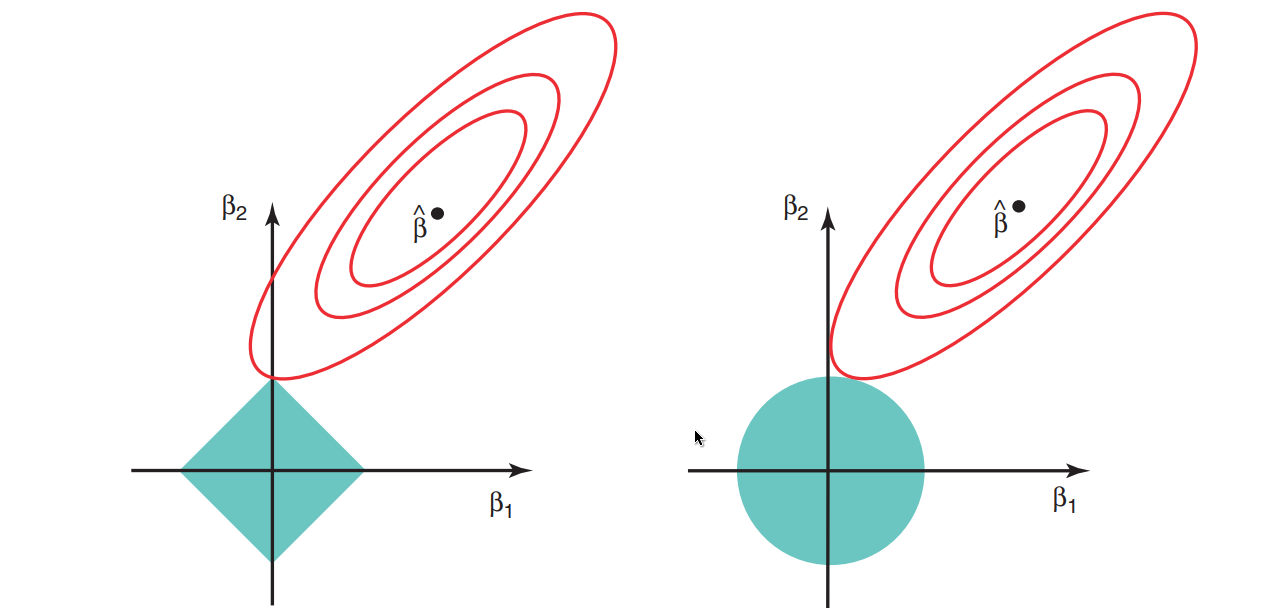
\includegraphics[width=1\linewidth]{Lasso_and_ridge.png}}
\caption{Границы ошибки $\sum_{i=1}^n(y_i - \sum_{j=1}^p \beta_j x_{ij})^2$ и ограничений  $\sum_{j = 1}^p |\beta_j| \leq s$ для Лассо (слева) и $\sum_{j = 1}^p \beta_j^2 \leq s$ для гребневой регрессии (справа).}
\end{figure}

\end{frame}


\begin{frame}
\frametitle{Сравнение гребневой регрессии и Лассо}
Рассмотрим простой случай, когда $n = p$ и $X$ --- диагональная матрица с $1$ на диагонали.

\textbf{МНК:}

\[\sum_{j =1}^p (y_j - \beta_j)^2.\]

\textbf{Решение гребневой регрессии:}
\[\hat{\beta}_{\lambda}^R = \frac{y_j}{1 + \lambda}.\]

\textbf{Решение Лассо:}
\begin{equation*}
\hat{\beta}_{\lambda}^L = 
 \begin{cases}
   y_j - \lambda/2, & \qquad y_j > \lambda/2\\
   y_j + \lambda/2, & \qquad y_j < -\lambda/2 \\
   0, & \qquad |y_j| \leq \lambda/2.
 \end{cases}
\end{equation*}



\end{frame}


\begin{frame}
\frametitle{Сравнение гребневой регрессии и Лассо}
\vspace{-0.3cm}

\begin{figure}
\center{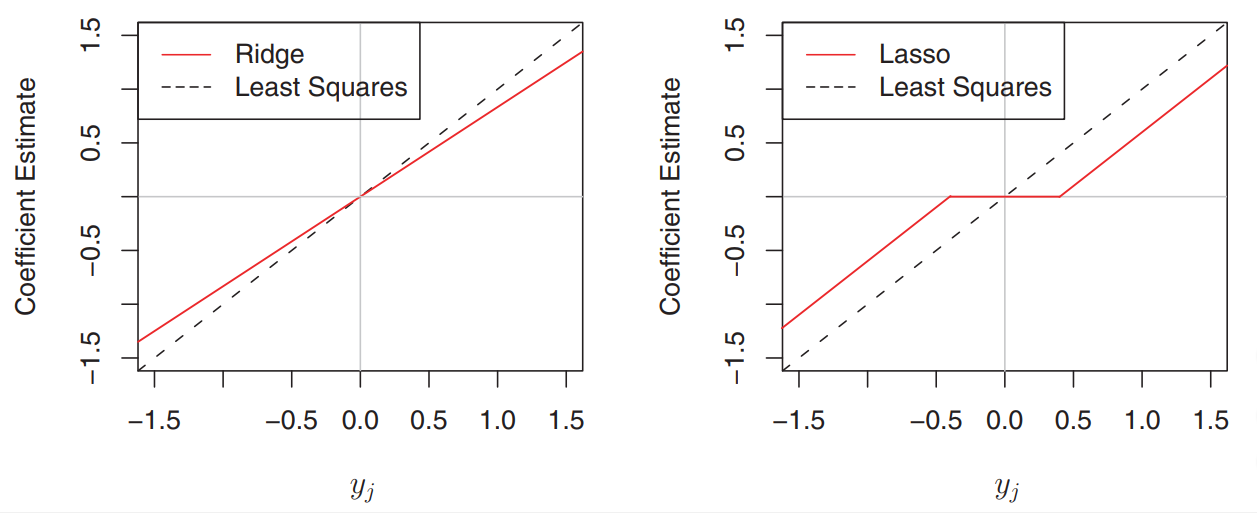
\includegraphics[width=1\linewidth]{compare.png}}
%\caption{Границы ошибки $\sum_{i=1}^n(y_i - \sum_{i=1}^p \beta_i x_i)^2$ и ограничений  $\sum_{j = 1}^p |\beta_j| \leq s$ для Лассо (слева) и $\sum_{j = 1}^p \beta_j^2 \leq s$ для гребневой регрессии (справа).}
\end{figure}
\vspace{-0.3cm}

\begin{itemize}
\item Гребневая регрессия уменьшает каждый коэффициент с равной пропорцией; 
\item Лассо уменьшает значения коэффициентов на одинаковое значение;
\item В Лассо, если коэффициент по модулю меньше $\lambda/2$, то его значение становится равным нулю.
\end{itemize}

\end{frame}

\begin{frame}
\frametitle{Сравнение гребневой регрессии и Лассо}

Нельзя выделить ни одну из моделей (Лассо или гребневая регрессия) как лучшую.

\vspace{0.8cm}
Можно ожидать, что 
\begin{itemize}
\item Лассо будет иметь ошибку меньше, когда в модели мало значимых признаков (коэффициенты при таких признаках будут равны нулю);
\item Гребневая регрессия будет иметь ошибку меньше, когда $Y$ будет зависеть от признаков, которые имеют примерно равную значимость. 
\end{itemize}

%\begin{itemize}
%\item Лассо будет иметь ошибку меньше, когда в модели мало информативных признаков;
%\item Гребневая регрессия будет иметь ошибку меньше, когда $Y$ будет зависеть от многих признаков, которые имеют примерно равные коэффициенты $\beta_j$. 
%\end{itemize}

\vspace{0.8cm}
С помощью кросс-проверки можно определить какой подход лучше.

\end{frame}

%Делает отбор информативных признаков, зануляет коэффициенты (показать почему, конец 221 стр ISLR)

%Когда лучше ридж, а когда наоборот? ( ISLR  стр 223-224 ) (когда мало информативных признаков лучше лассо)

%Ни ридж, ни лассо не являются лучшим алгоритмом!!!


\end{document}